\chapter{Introduction}
\label{chap:intro}
\minitoc

\nomenclature{DTI}{Diffusion Tensor Imaging}

 
 
 \section{Le domaine du Calcul Haute Performance} 
 

%---------------------------------------------------------------------------------

 \subsection{Le calcul scientifique et la simulation numérique}

Pour comprendre d'où émerge le domaine du Calcul Haute Performance (HPC) il faut comprendre pour répondre à quels besoins ces architectures sont mises au point. 
Le domaine du calcul scientifique et notamment celui de la simulation numérique qui nécessite de granges puissances de calculs. Les simulations sont utilisées dans différents domaines car elles apportent beaucoup d'avantages. Le premier est la réduction des couts. Par exemple dans l'industrie automobile, les tests de crash de voiture ne sont plus réalisé avec de vrais voitures. Les voitures sont maintenant simulées et envoyées percuter des murs virtuels. Cette techniques à pour effet de réduire les temps de conception, car il n'y plus besoin de créer une voiture avec les matériaux à tester, et donc de réduire les couts de conceptions. Mais la simulation numérique à d'autres avantages, comme celui de pouvoir simuler des phénomènes dont les conditions ne sont pas reproductibles sur terre. Elle élargi donc les domaines explorable ce qui rend son champs d'application presque infini. Les domaines d'applications sont donc nombreux, on retrouve la simulation numérique dans la recherche pétrolière (analyse des fonds marins), les prévisions météoroligiques, en biologie (séquençage ADN) ou encore en finance.

\begin{figure}[H]
    \center
    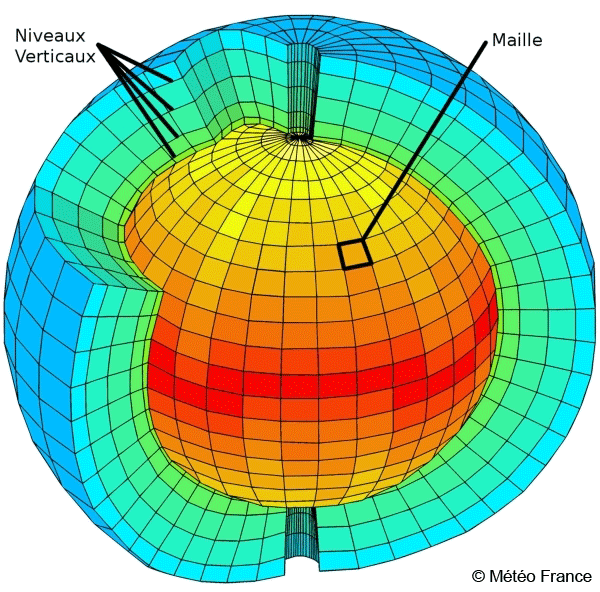
\includegraphics[width=4cm]{images/Chapitre1/maillage.png}
    \caption{\label{maillage} Le maillage le plus fin exploité par Météo-France pour ses prévisions régionales restitue des mailles de 2,5 km de côté. (source www.irma-grenoble.com)}
\end{figure}


Ces simulations numériques utilisent une réprésentation discrète des objets modélisés. Pour améliorer ces simulations, ces réprésentation doivent utiliser des maillages le plus fin possible. C'est en cela que ces simulations necessitent d'énormes puissances de calculs et que cette demande est casi illimité, car les maillages pourront toujours etre affinés. 


%---------------------------------------------------------------------------------

\subsection{Définition du Calcul Haute Performance}
\nomenclature{HPC}{Calcul Haute Performance}
 
Le domaine du Calcul Haute Performance est l'interconnexion de ressources informatiques dans le but de résoudre de façon partagée un problème complexe. Les probleèmes qui sont résolus grâce à ces immenses systemes sont très variés et interviennent dans de nombreux domaines. Le point commun de ces application est la résolution d'un gros problème qui ne peut pas être résolu par une seule ressource. Ce problème est divisé en sous-problème de petites tailles, qui eux peuvent être résolus séparément. Cette mêthode de résolution est appelée le calcul pralallele (voir ??). 
Aujourd'hui il existe trois façon d'apporter cette puissance de calcul aux utilisateurs:
\begin{enumerate}
\item \textbf{Dedicated supercomputer}, unique est créee ce qui rend son prix très cher. Ces architectures ne sont utilisées que très rarement aujourd'hui pour des cas très précis.
\item \textbf{Commodity cluster}, qui agrège du matériel grand public pour former des grappes de calculs de plusieurs milliers de processeurs.
\item HPC dans le nuage, TODO avec Poru les nuls
\end{enumerate}

Ce regroupements de centaines, voire de milliers de ressources forme une grappe de serveur que l'on appelle un \textit{cluster} ou \textit{supercalculateur}.


\subsection{Les Clusters}
A l'origine les premiers supercalculateurs étaient des architectures uniques crées de toutes pièces pour un client. Il était alors très dure de les reproduire ensuite rendant leur cout de conception trés élevé. Seymour Cray présenta le premier super- calculateur en 1960 alors qu'il travaillait pour Control Data Corporation. A partir des années 1990 apparurent des clusters construits à partir de materiels, certes haut de gamme, mais qui constituent les ordinateurs grand public. C'est seulement le regroupement de centaines de stations de travail qui en fait des supercalculateur, et cette façon de les construire est toujours la même aujourda'hui.

\cite{Ste95}


\subsection{Loi de Moore A DEPLACER}
En 1965, Gordon Moore fit l'une des prédictions les plus visionnaires de toute l'histoire de l'informatique (Moore, 1965) lorsqu'il énonça que la performance des ordinateurs doublerait tous les dix-huit mois. De nos jours, cette remarquable prédiction reste toujours aussi pertinente. Cependant, alors que cette amélioration des performances a longtemps permis de conserver un modele de programmation sequentiel, ces dernieres années ont vu apparaitre des sarchitectures parallèles au sein même des microprocesseurs (multicoeurs). Ce changement de conception radical au niveau du matériel, oblige à revoir les méthodes de développement logiciel afin de tirer pleinement parti de la puissance de ces nouveaux processeurs.

